\chapter{Design and Implementation}
\label{chapter:design-implementation}



CEVA TEXT AICI

\begin{figure}[H]
    \centering
    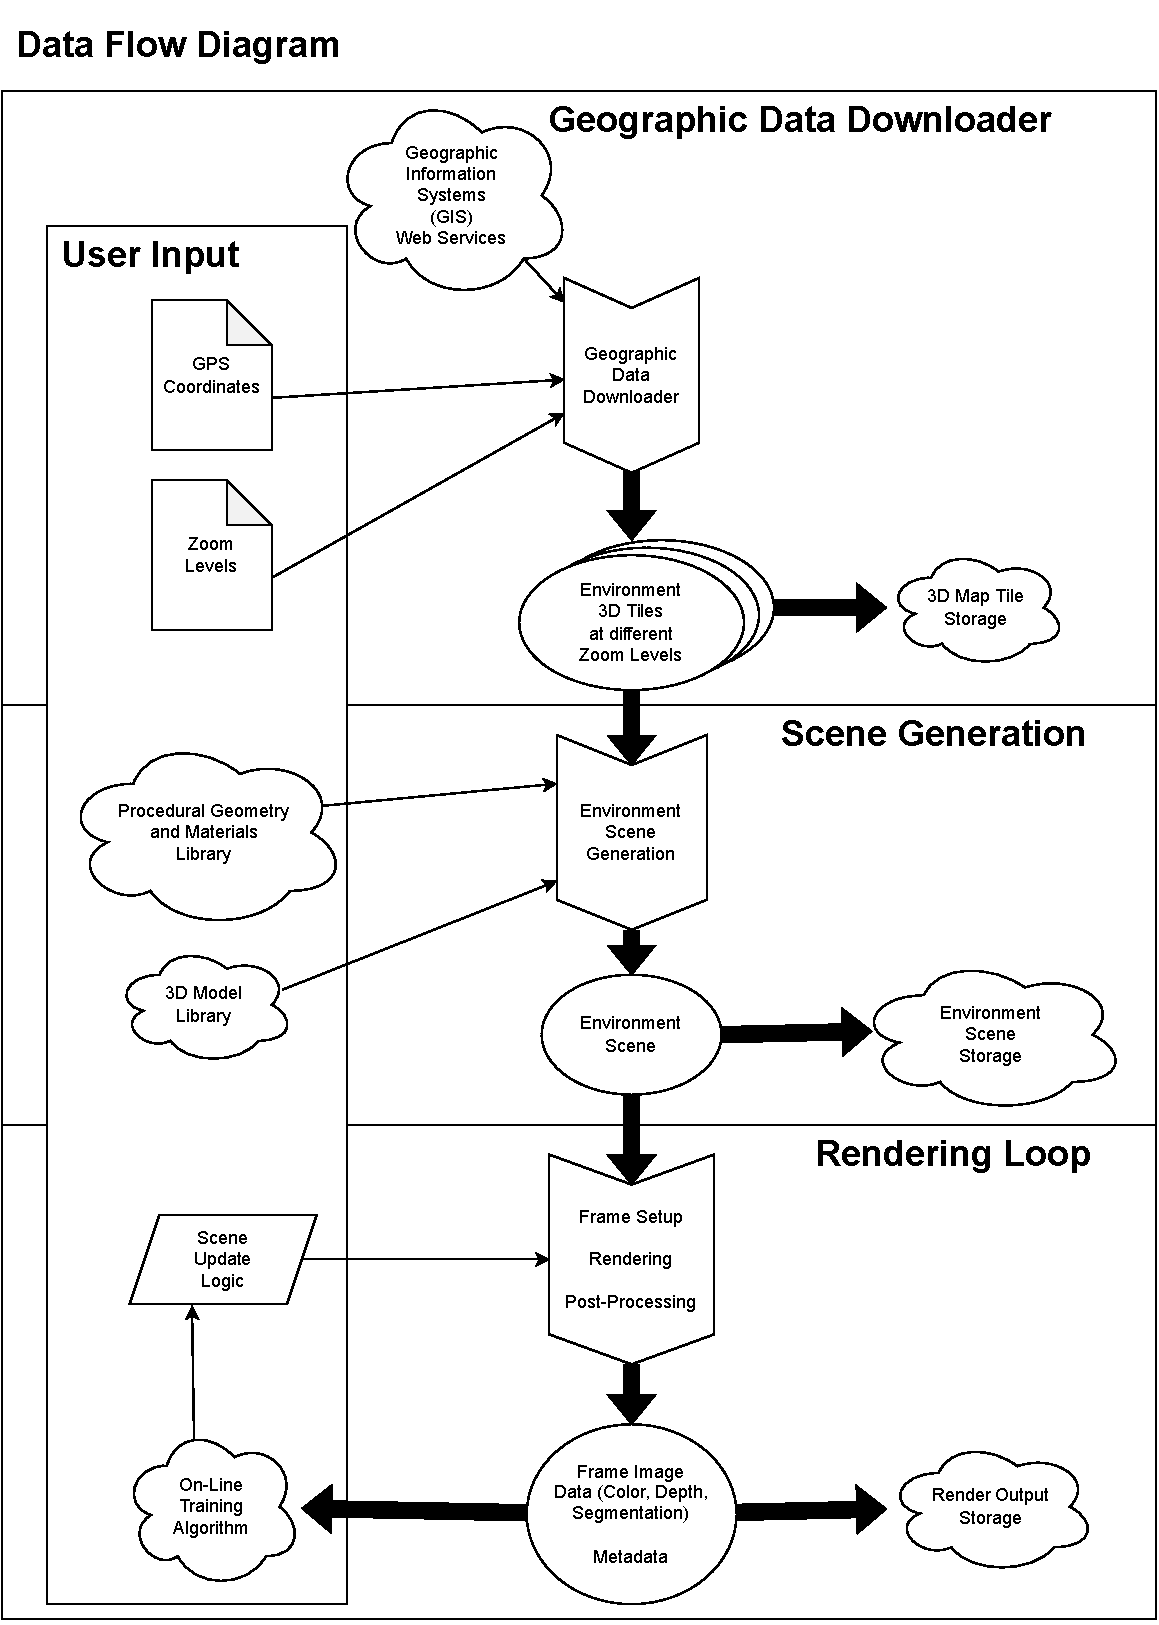
\includegraphics[width=14.5cm]{src/img/fig/fig-1-overview-v2.drawio-1.pdf}
    \caption{Data Flow Diagram}
    \label{fig:design-overview}
\end{figure}


CEVA TEXT AICI

\section{Design}
\label{sec:design}


CEVA TEXT AICI

\begin{figure}[H]
    \centering
    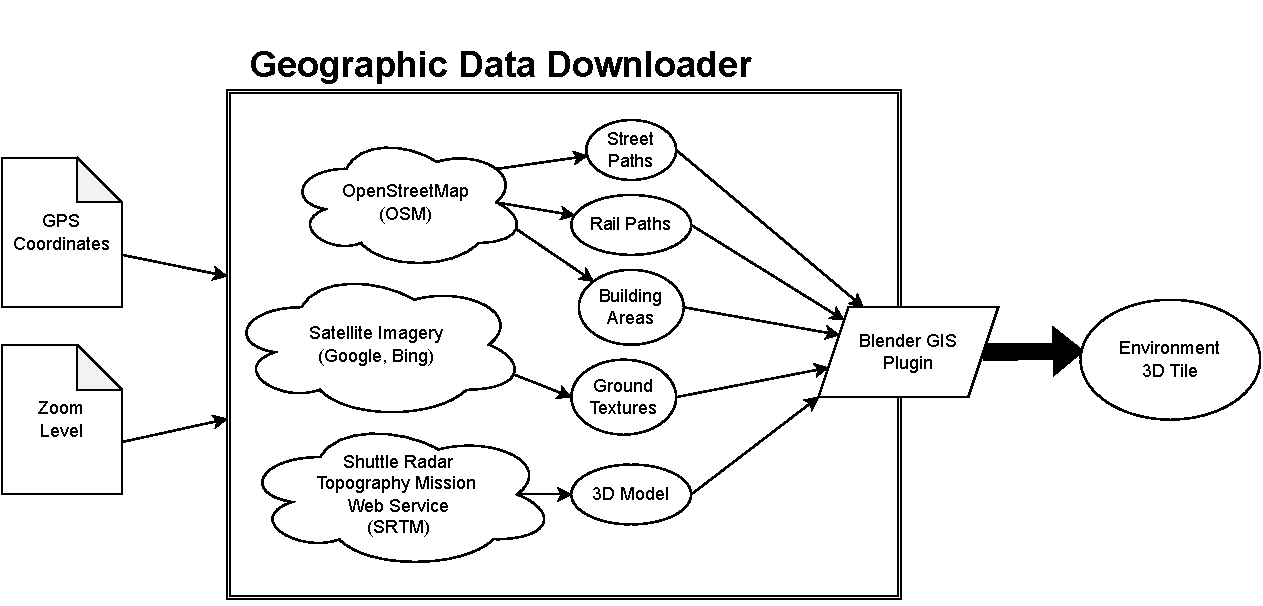
\includegraphics[width=14.5cm]{src/img/fig/fig-2 Geographic Data Downloader.drawio.pdf}
    \caption{Geographic Data Downloader}
    \label{fig:design-data-downloader}
\end{figure}


CEVA TEXT AICI

\begin{figure}[H]
    \centering
    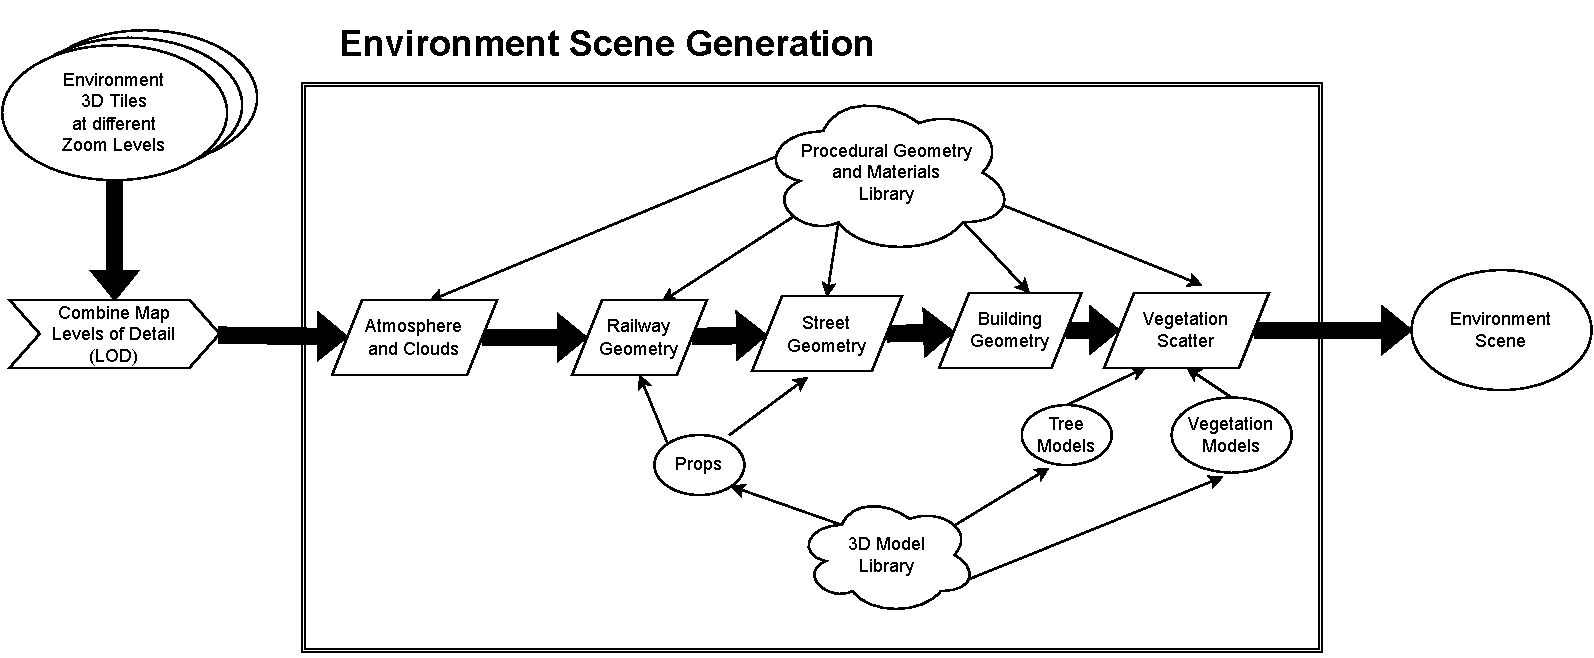
\includegraphics[width=14.5cm]{src/img/fig/fig-3 environment scene generation.drawio.pdf}
    \caption{Scene Generation}
    \label{fig:design-scene-generation}
\end{figure}

CEVA TEXT AICI

\begin{figure}[H]
    \centering
    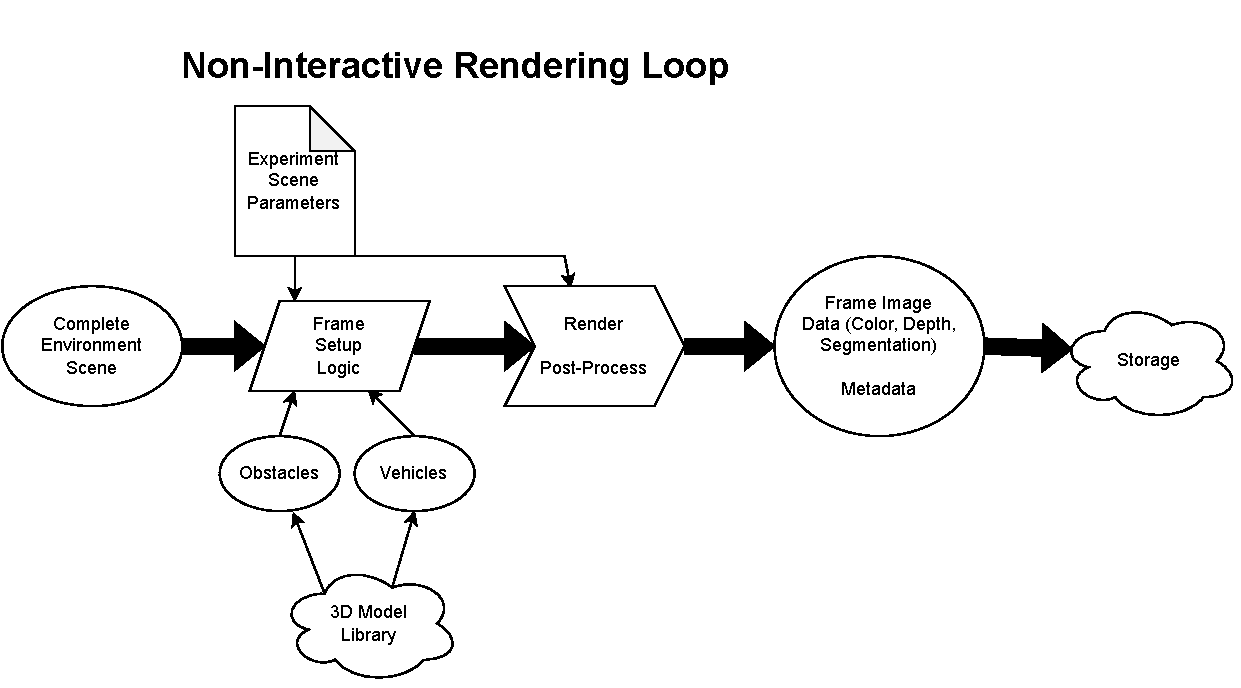
\includegraphics[width=14.5cm]{src/img/fig/fig-4 non-interactive render loop.drawio.pdf}
    \caption{Simple Render Loop}
    \label{fig:design-render-non-interactive}
\end{figure}


CEVA TEXT AICI

\begin{figure}[H]
    \centering
    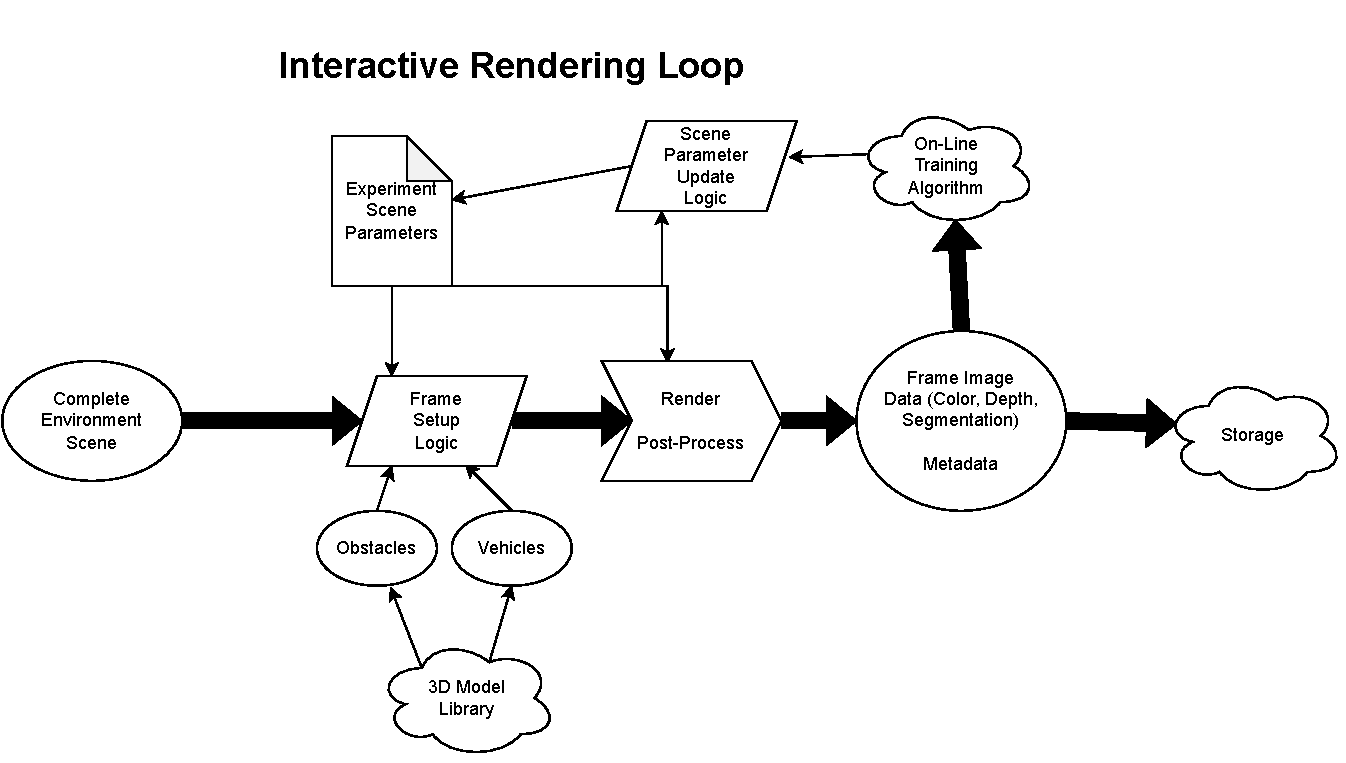
\includegraphics[width=14.5cm]{src/img/fig/fig-5 interactive render loop.drawio.pdf}
    \caption{Interactive Render Loop}
    \label{fig:design-render-interactive}
\end{figure}


CEVA TEXT AICI



\section{Implementation}
\label{sec:implementation}


CEVA TEXT AICI

\begin{figure}[H]
    \centering
    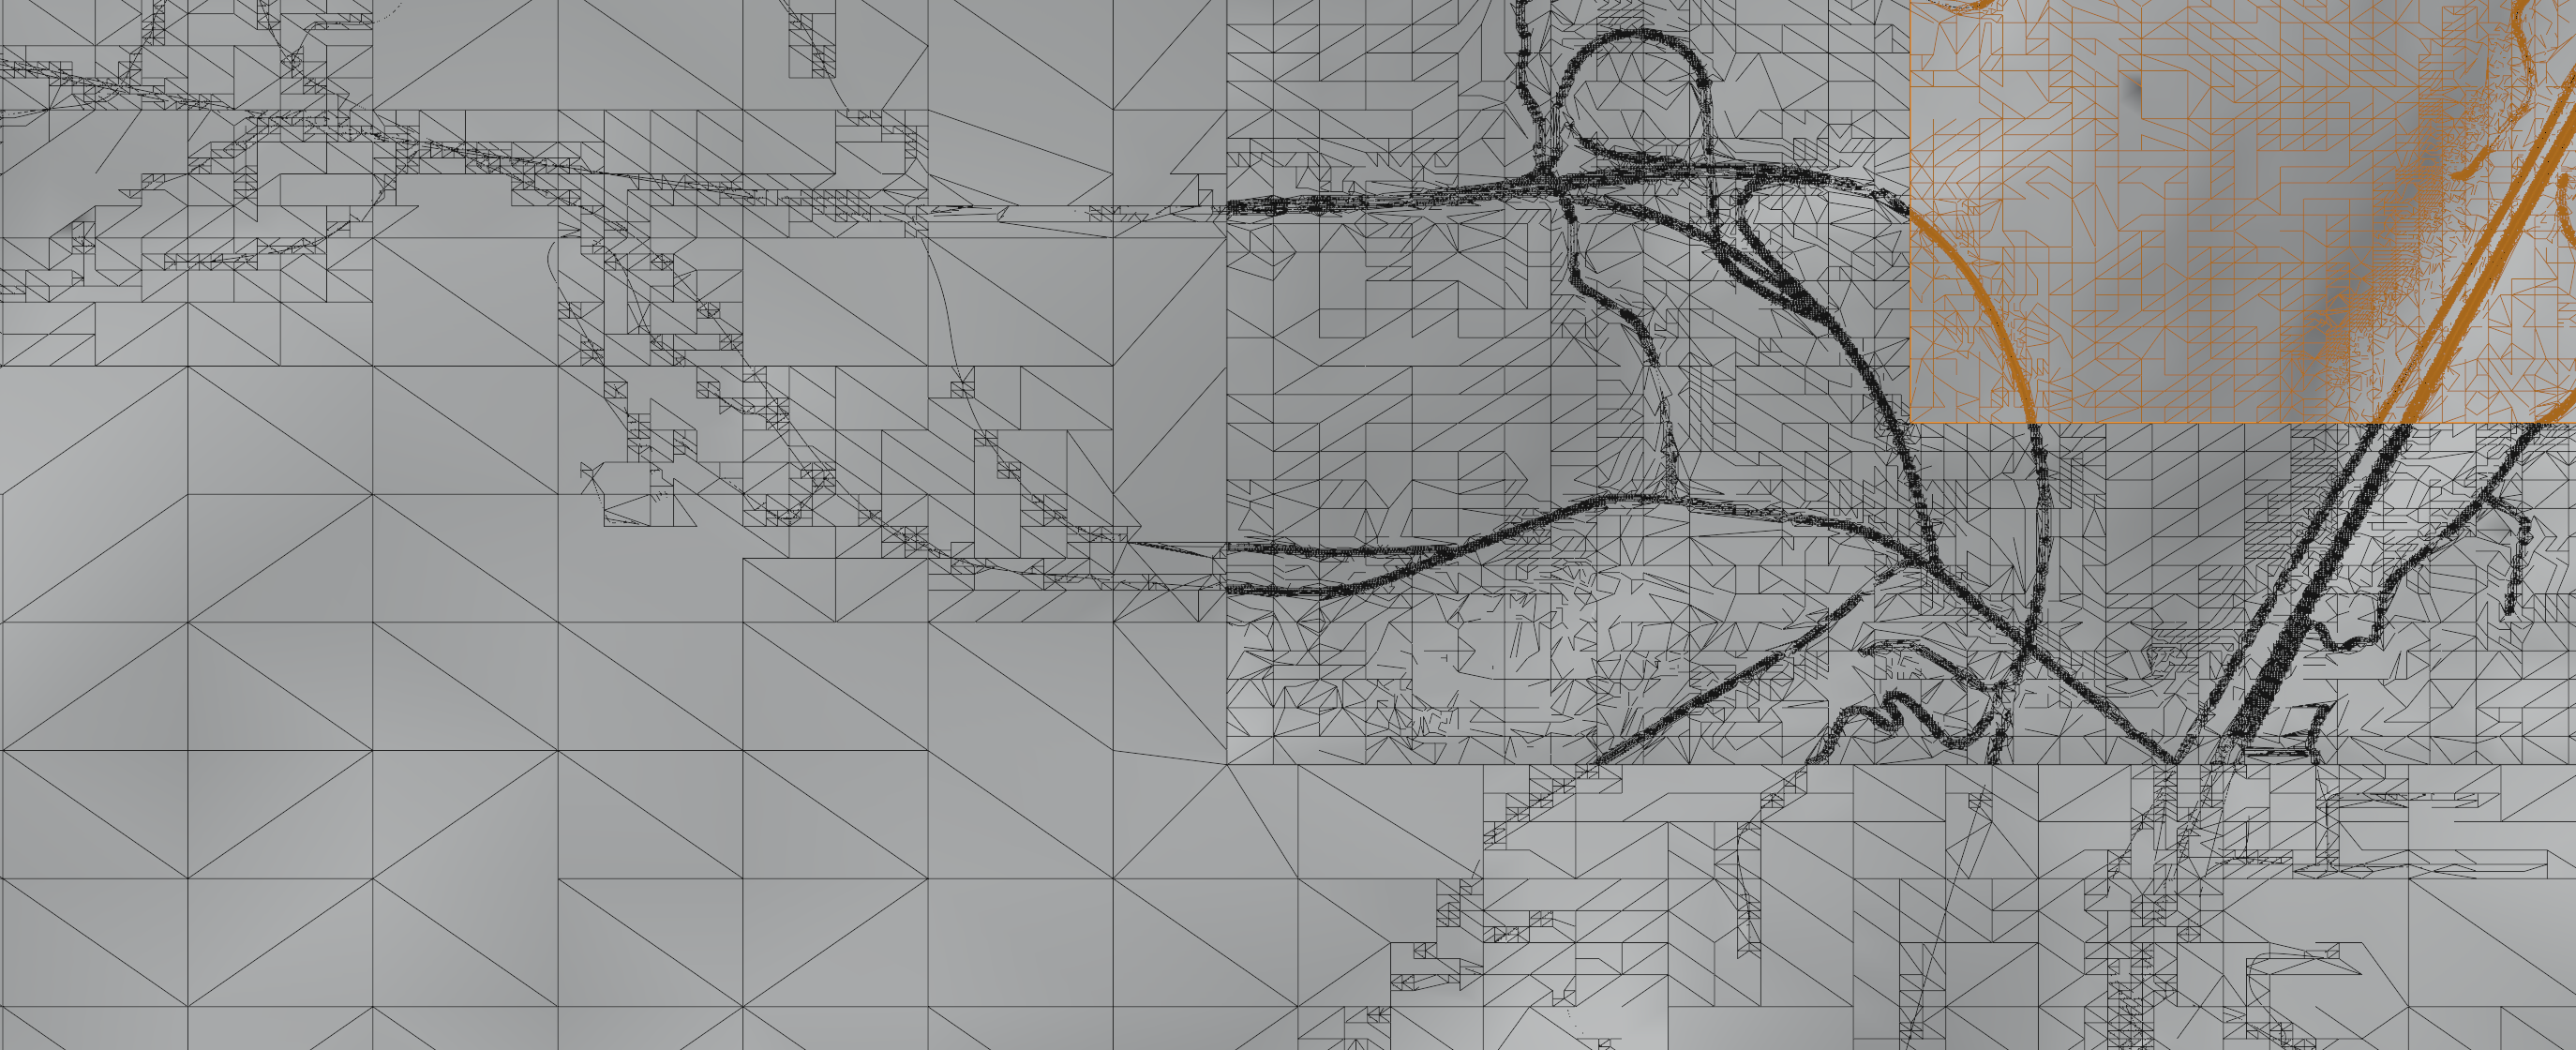
\includegraphics[width=14.5cm]{src/img/pic/pic-1 blender screenshot sat levels of detail.png}
    \caption{Different levels of detail }
    \label{fig:design-render-interactive}
\end{figure}


CEVA TEXT AICI

\begin{figure}[H]
    \centering
    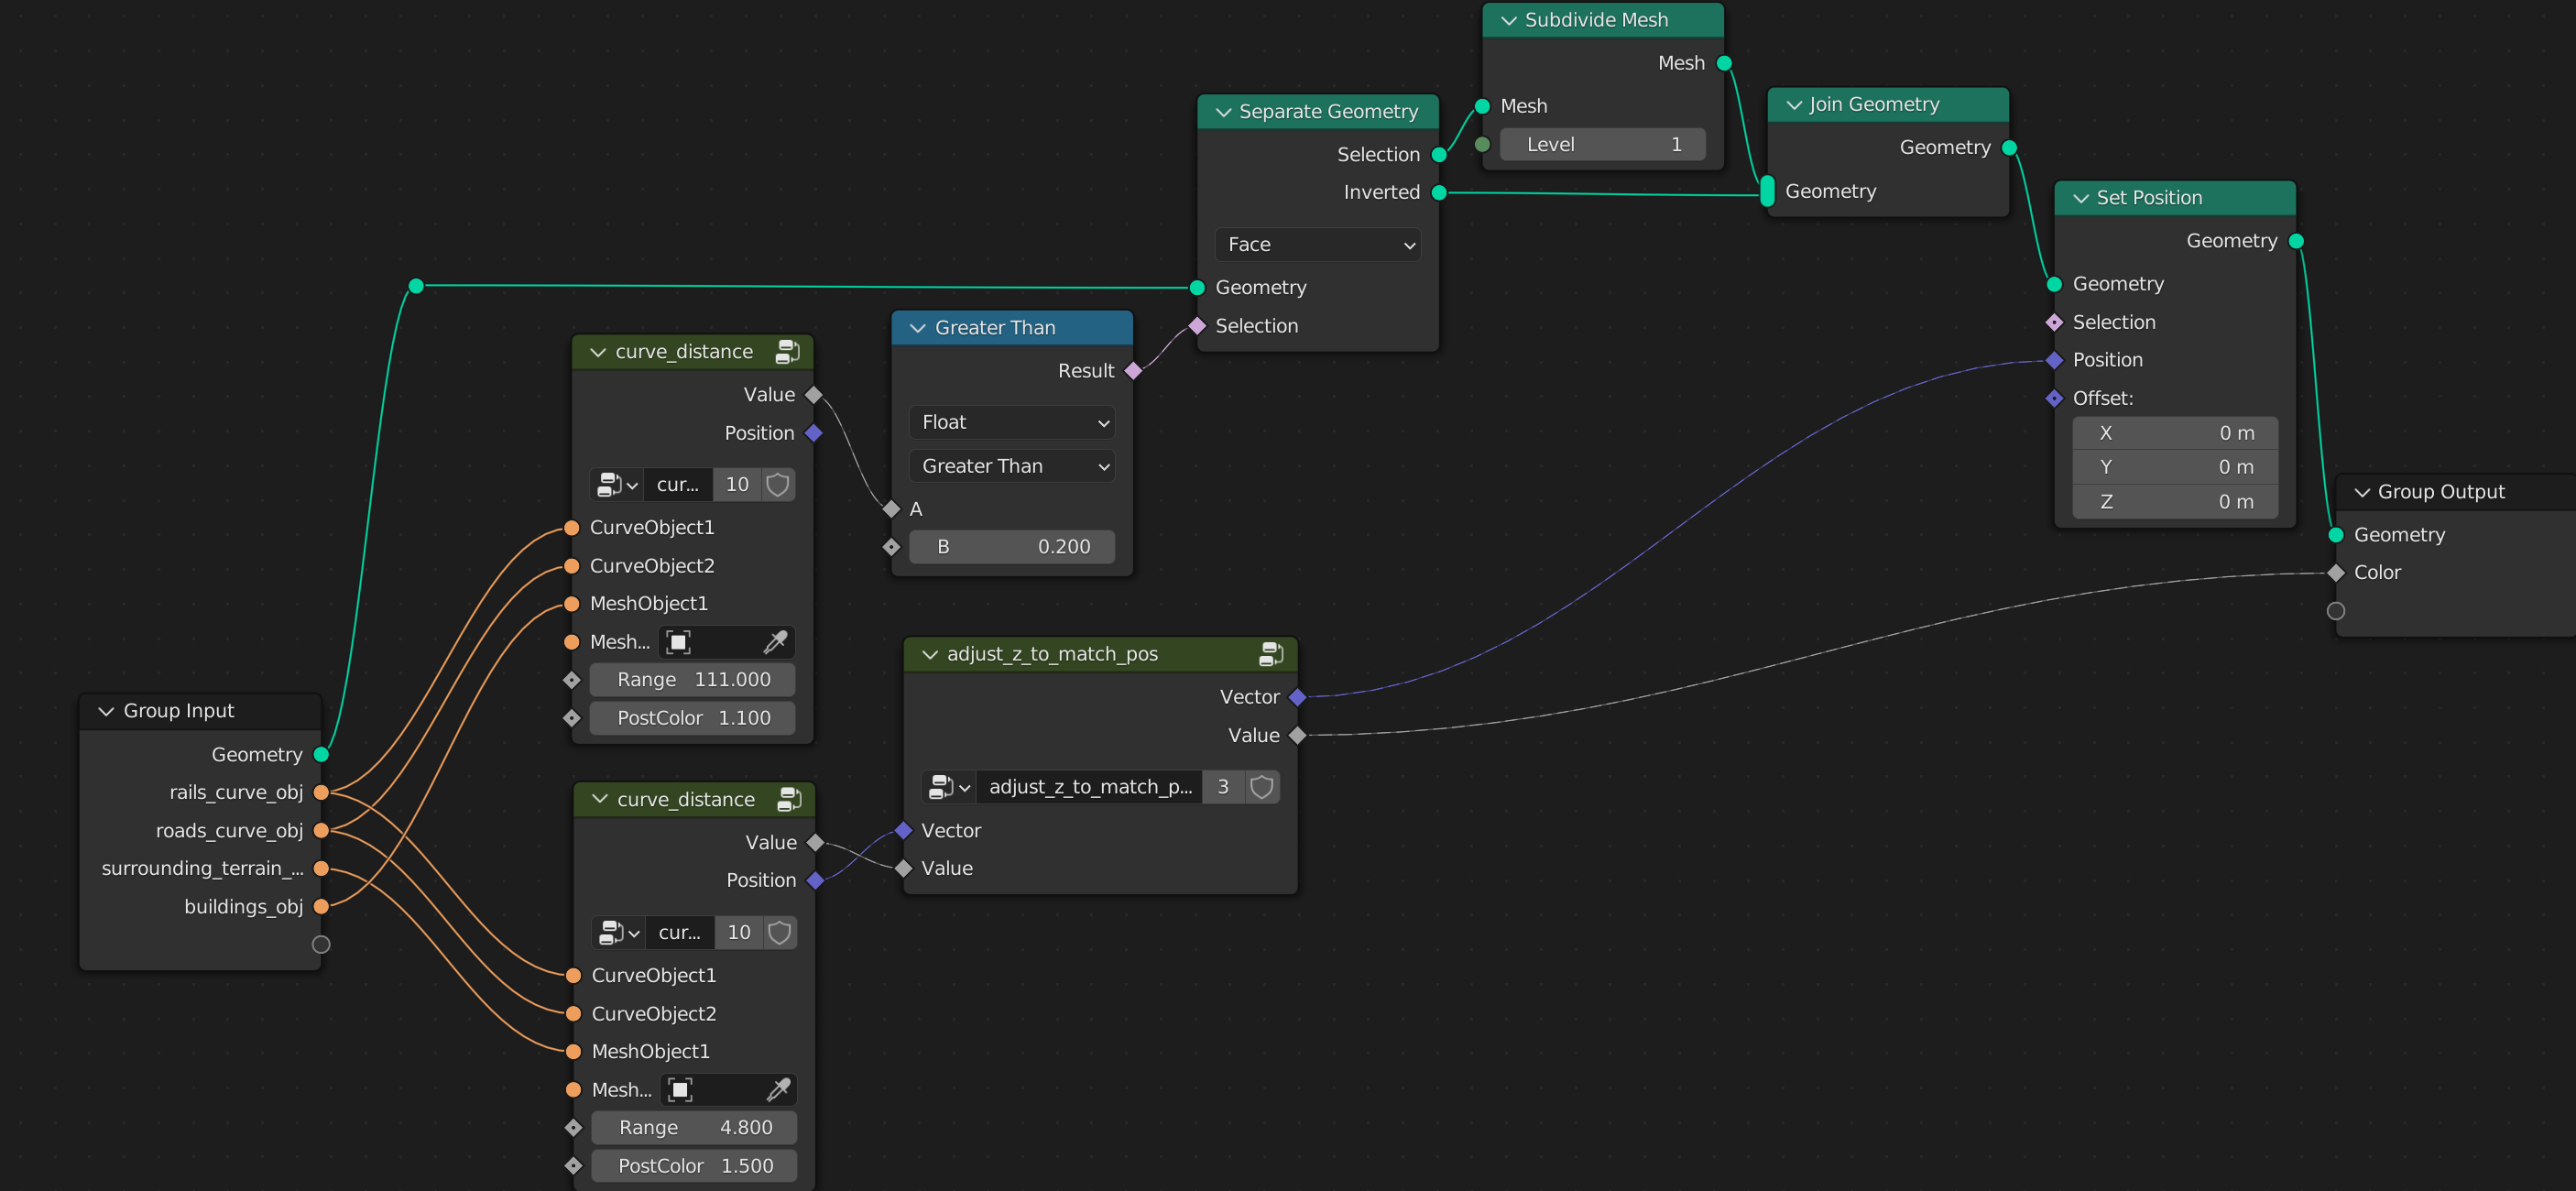
\includegraphics[width=14.5cm]{src/img/pic/pic-2 screenshot of blender adjust terrain geometry node.png}
    \caption{Geometry Node Implementation for terrain height adjustment and tesselation}
    \label{fig:design-render-interactive}
\end{figure}


CEVA TEXT AICI


\begin{figure}[H]
    \centering
    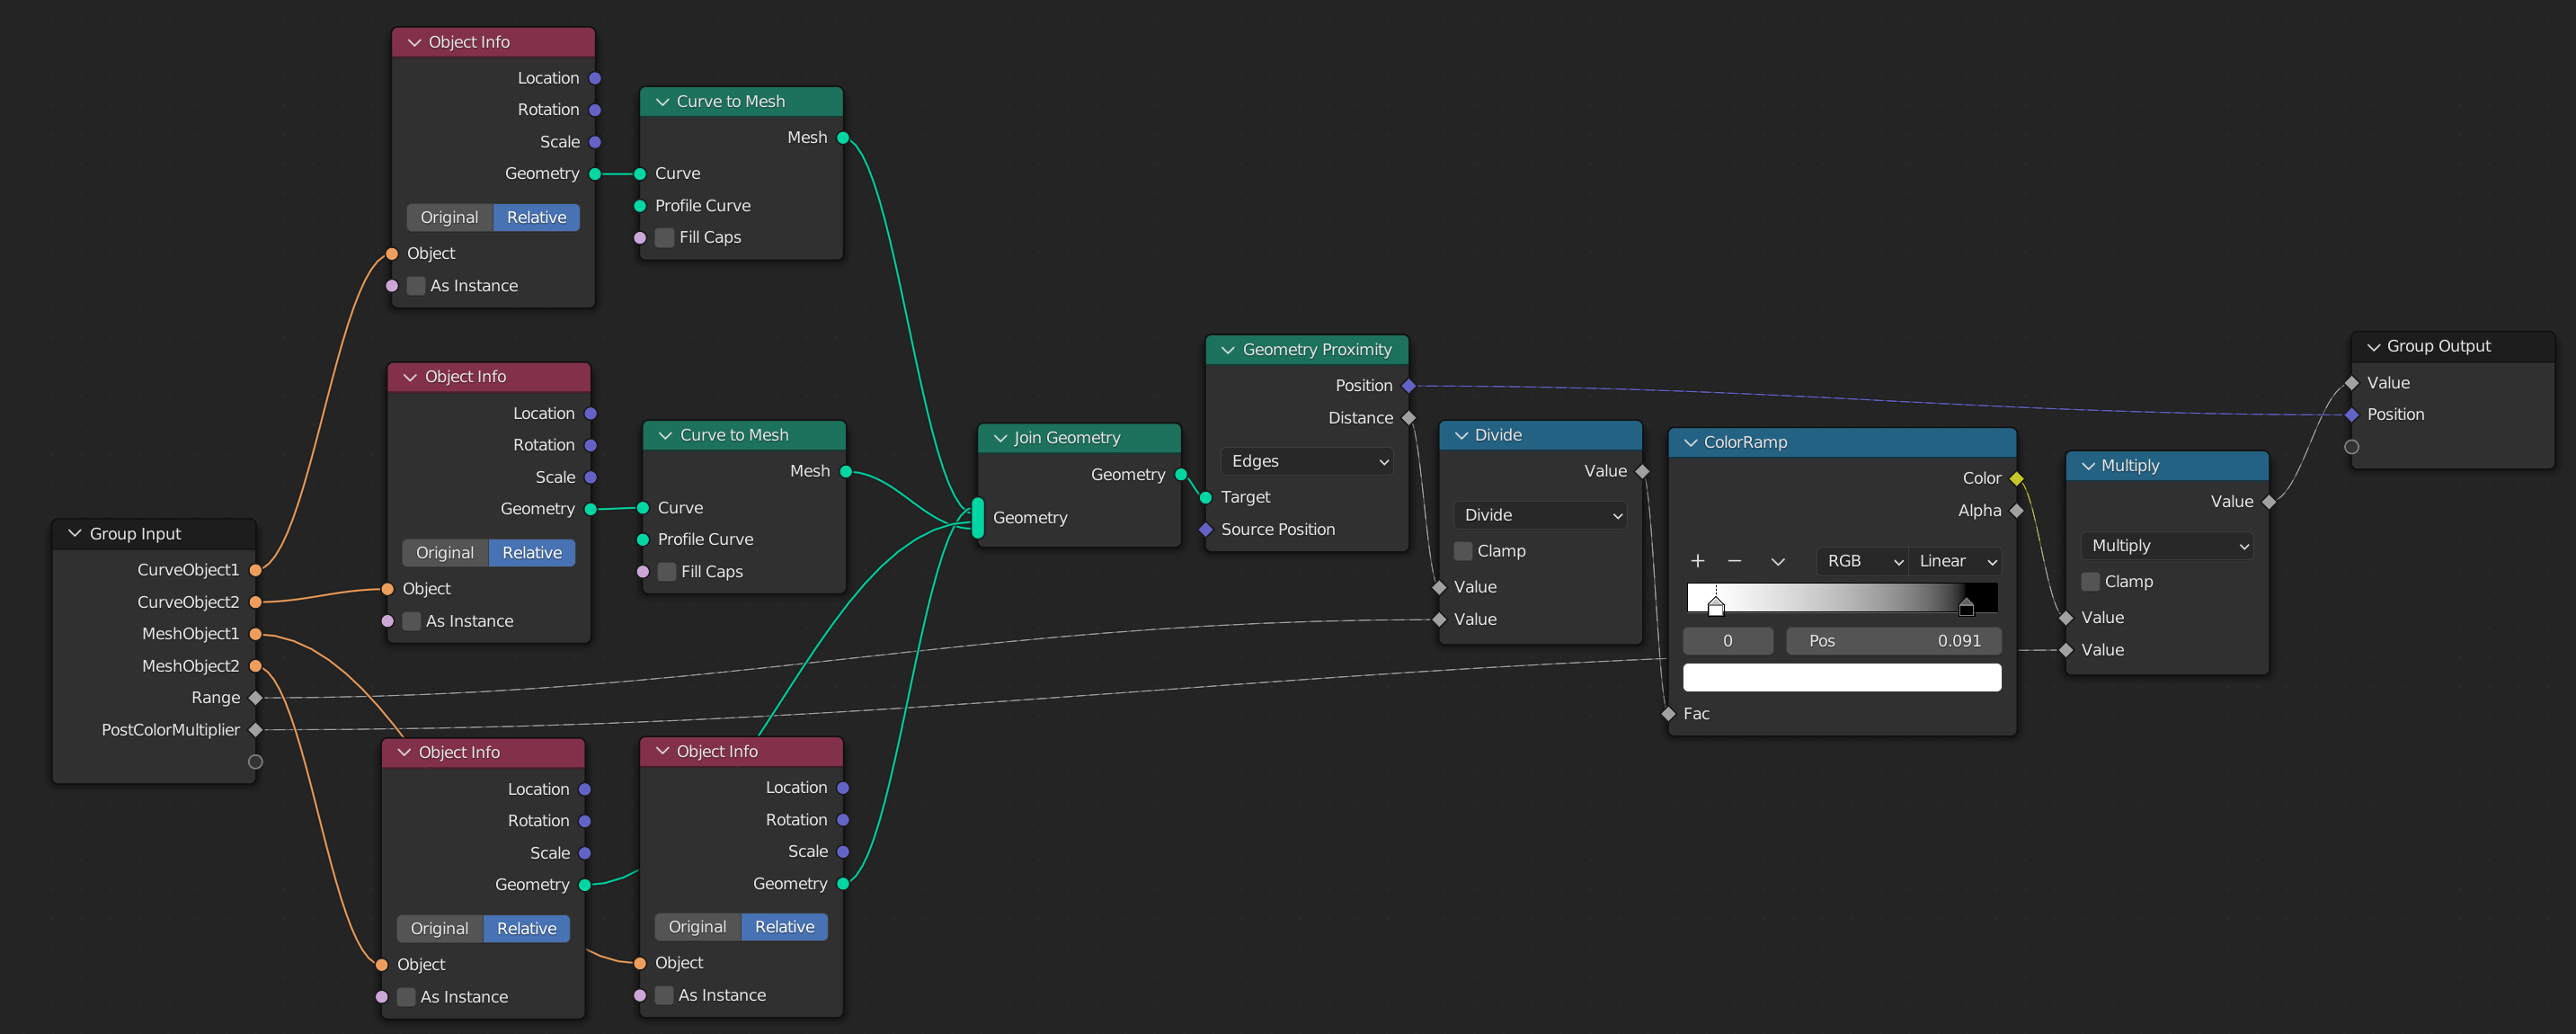
\includegraphics[width=14.5cm]{src/img/pic/pic-3 blender geometry screenshot curve_distance.png}
    \caption{Geometry Node Implementation for curve_distance}
    \label{fig:design-render-interactive}
\end{figure}
\begin{figure}[H]
    \centering
    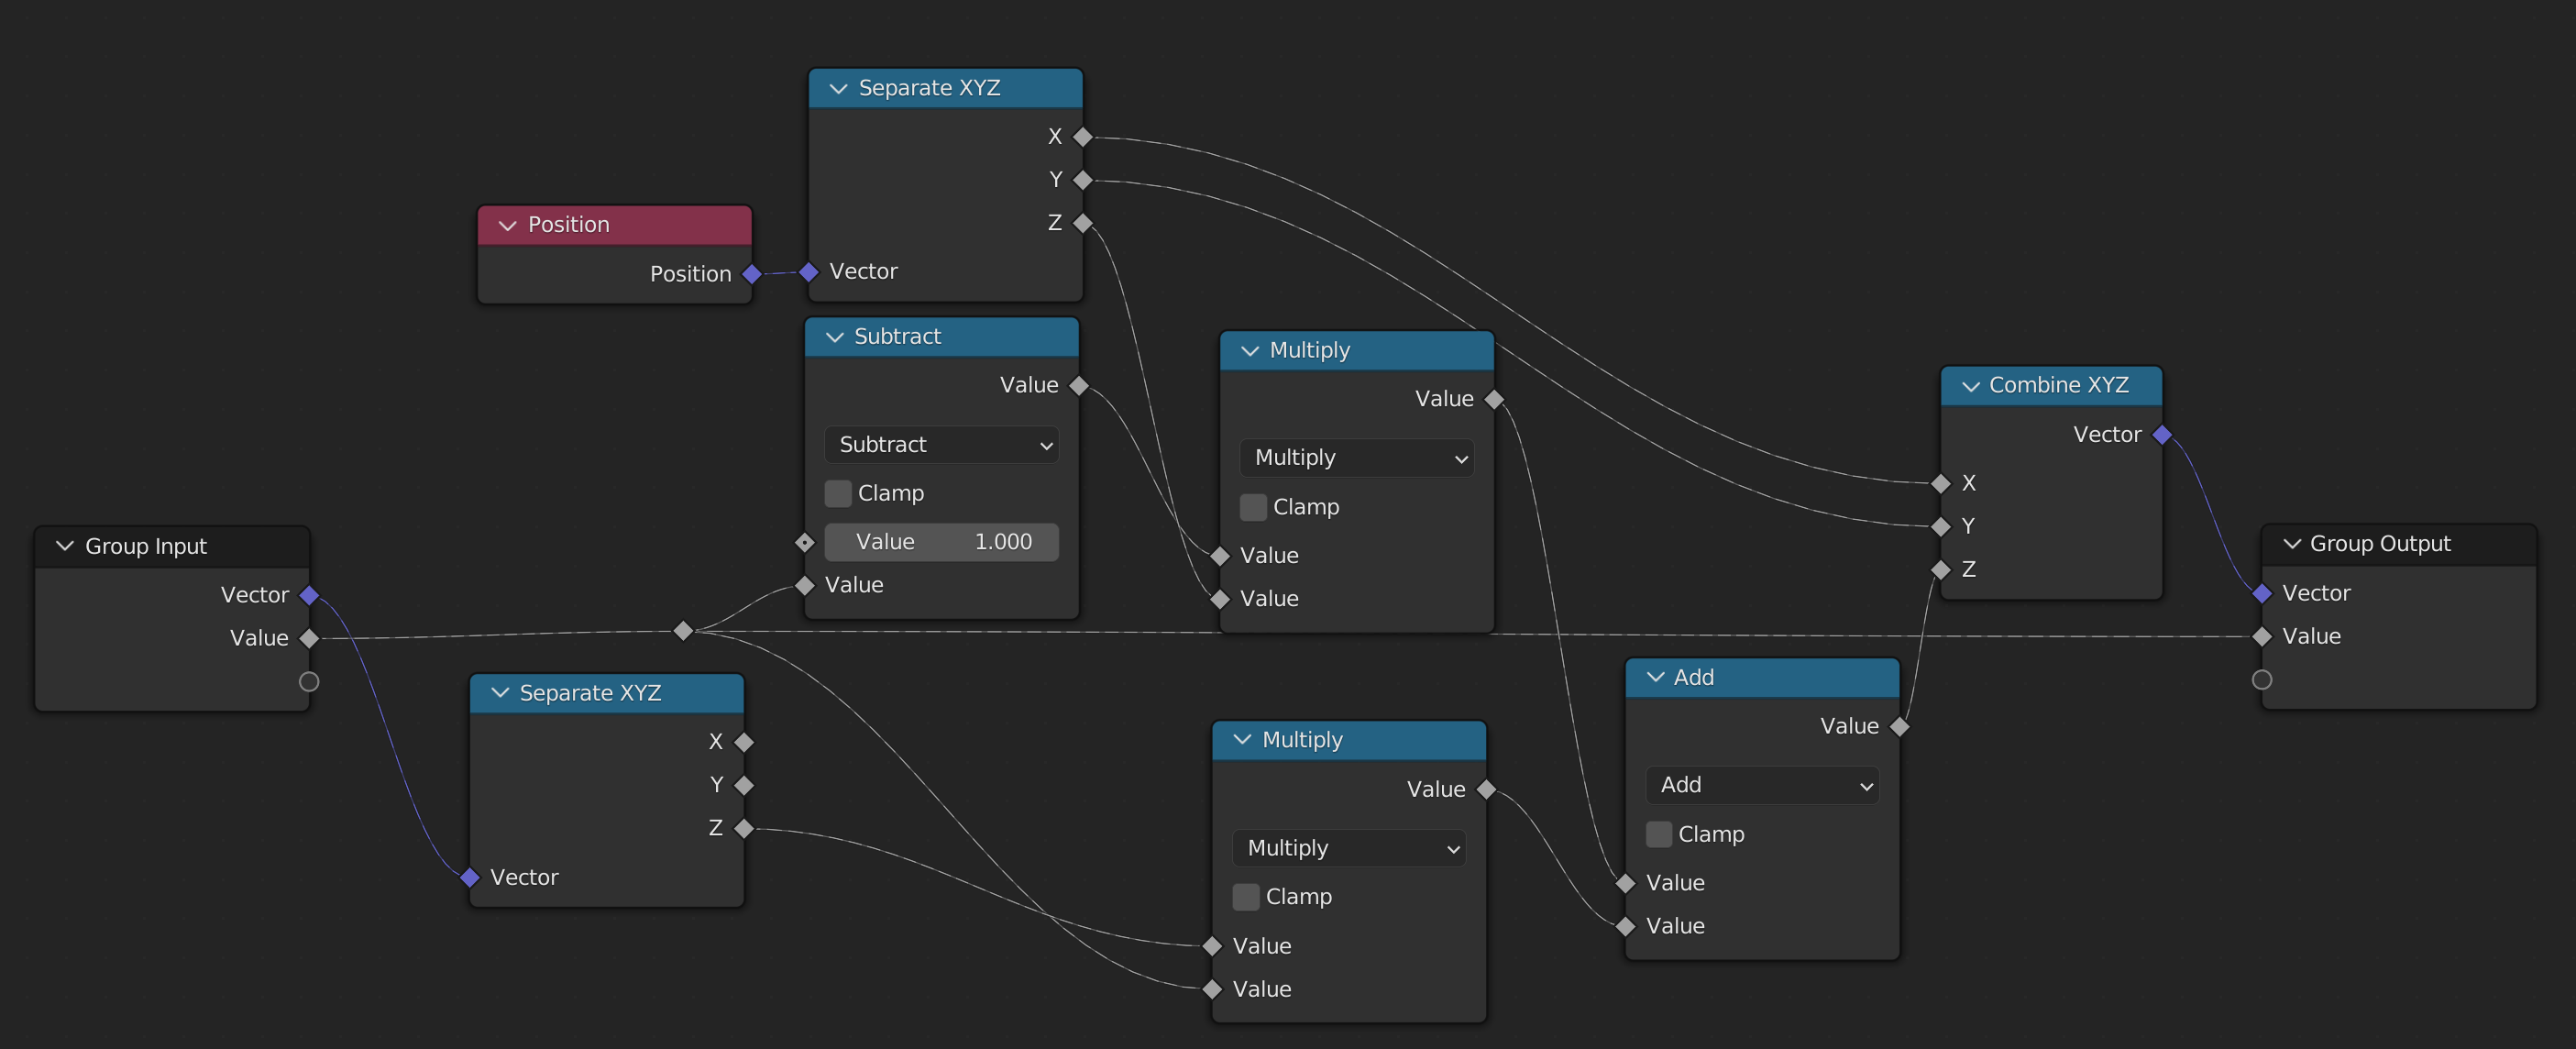
\includegraphics[width=14.5cm]{src/img/pic/pic-4 blender geometry node screenshot adjust_z_to_match_pos.png}
    \caption{Geometry Node Implementation for adjust_z_to_match_pos}
    \label{fig:design-render-interactive}
\end{figure}


CEVA TEXT AICI

\section{Testing}
\label{sec:testing}
